\documentclass{beamer}


% Vary the color applet  (try out your own if you like)
\colorlet{structure}{red!65!black}

\beamertemplateshadingbackground{yellow!100}{white}

\usepackage{beamerthemesplit}
\usepackage{graphics}
\usepackage{graphicx}
\usepackage{hyperref}
\usepackage{pifont}
\usepackage{cancel}
\usepackage{ulem}
\usepackage{listings}

\newcommand{\tabincell}[2]{\begin{tabular}{@{}#1@{}}#2\end{tabular}}

\title[Congestion Control Mechanisms for OBS Networks]{Congestion Control Mechanisms for \\ Optical Burst Switched \\ Networks}

\author[Fei Wang]{%
\hspace{-10mm}Author: Fei Wang \\
    Supervisor: Dr. Conor McArdle \\
    \hspace{22mm}Prof. Tommy Curran
}

\institute[Dublin City University]{
  Faculty Of Engineering \& Computing\\
  Dublin City University}

\date[\today]{\today}
\subject{M.Eng. in Telecommunications Engineering}

\pgfdeclaremask{dcu}{dcu_logo_scale}
\pgfdeclareimage[mask=dcu,width=1cm]{dcu-logo}{dcu_logo_scale}

\logo{\vbox{\vskip0.1cm\hbox{\pgfuseimage{dcu-logo}}}}

\begin{document}

  \frame
  {
    \titlepage
  }

  \section*{Outline}

  \frame
  {
    \frametitle{Outline of Topics}

    \tableofcontents
  }

  \section{Optical Burst Switching Technique}

  \frame
  {
    \frametitle{Why OBS?}
	$d_{packet} = {\xcancel{d_{proc}}} + {\xcancel{d_{queue}}} + d_{prop}+\uuline{d_{trans}}$
	\vskip+2em
    \begin{tabular}{|l|l|l|l|l|}
    \hline
    \tabincell{l}{Optical \\ Switching \\ Paradigm} & \tabincell{l}{Bandwidth \\ utilization} & \tabincell{l}{Latency} & \tabincell{l}{Implemetation \\ difficulty} & \tabincell{l}{Adaptivity} \\
    \hline
    Wavelength & Low & High & Low & Low \\
    \hline
    Packet/Cell & High & Low & High & High \\
    \hline
    OBS & High & Low &  Medium & High  \\
    \hline
    \end{tabular}
    \vskip+2em
    OBS is fast becoming an important area of research.
  }

  \frame
  {
    \frametitle{How OBS work?}
    \begin{figure}
      \scalebox{0.25}
      {
        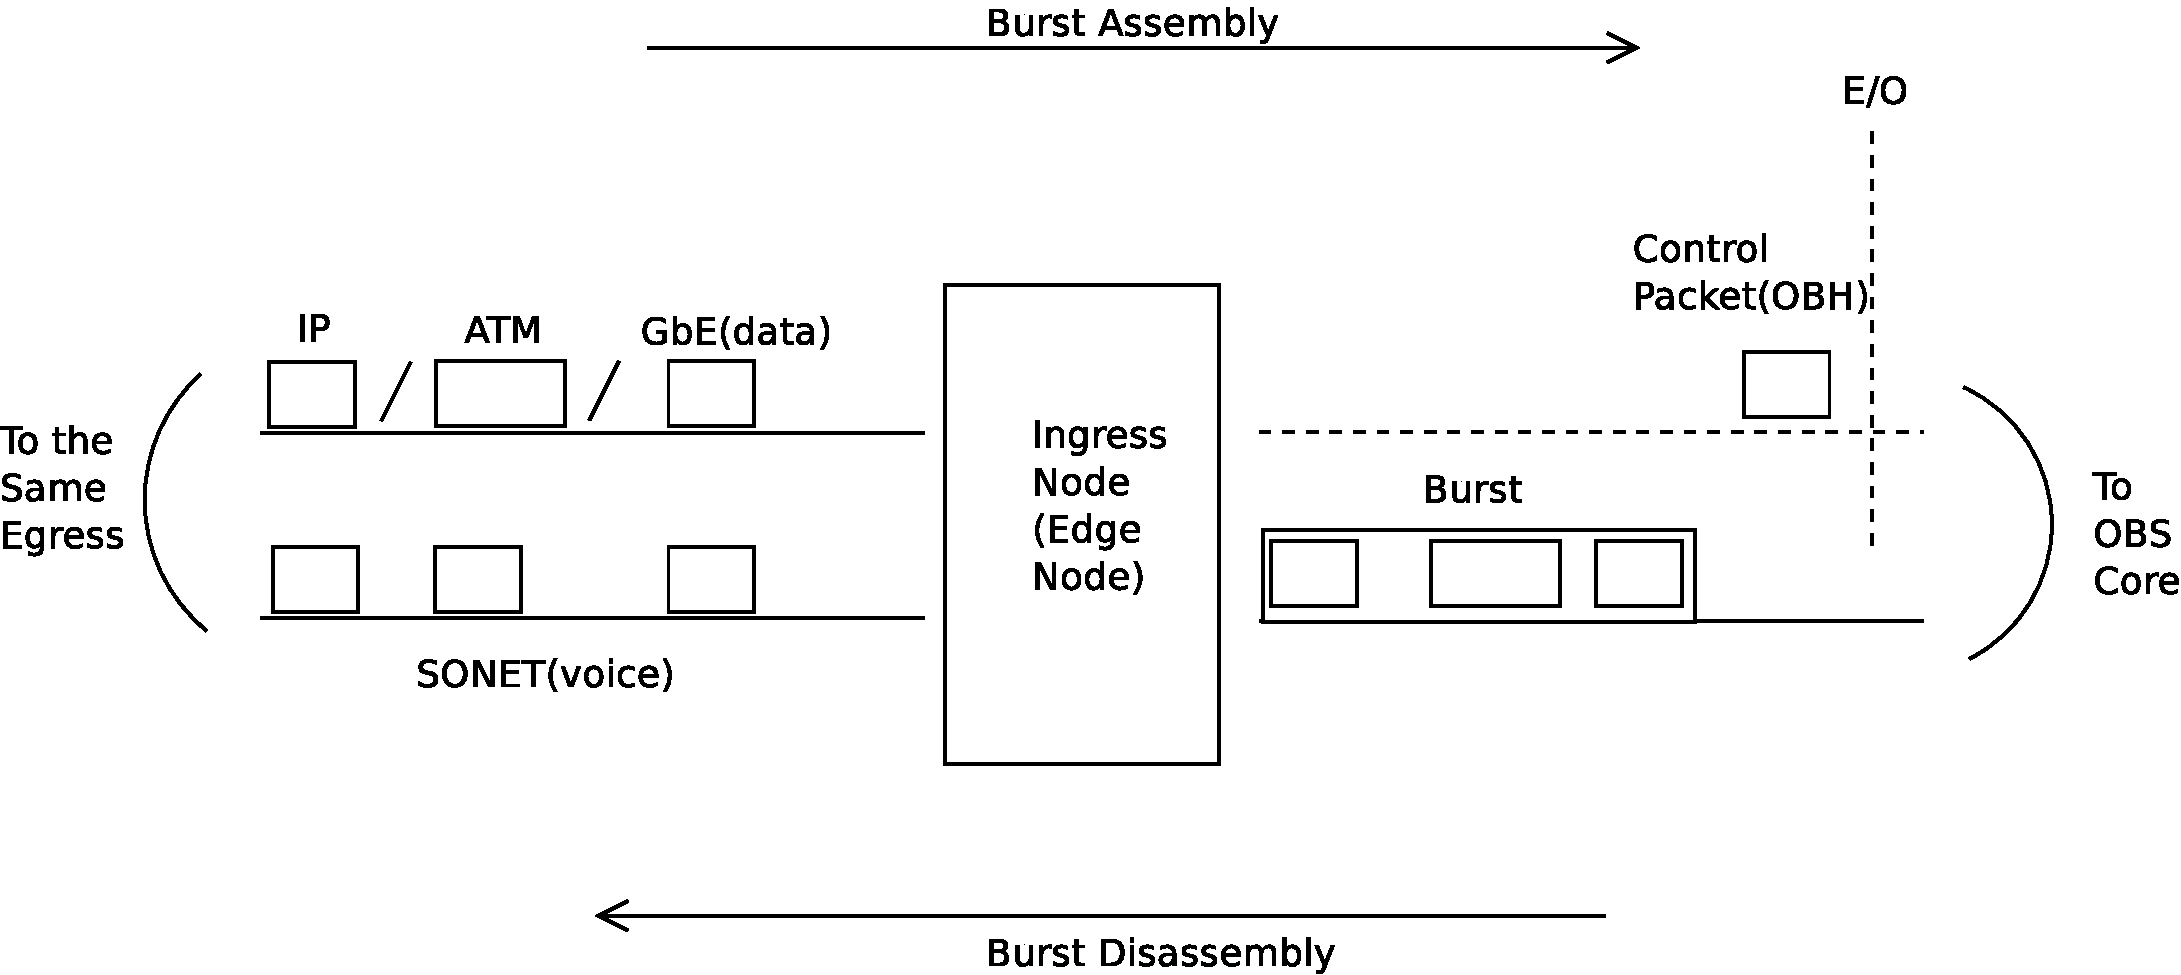
\includegraphics{obs_work.pdf}
      }
    \end{figure}

    From this figure, we can learn that the load control could be done {\bf only} by the {\bf edge nodes} since they have more intelligence and adequate physical resources.
  }


  \frame
  {
    \frametitle{OBS vs. Circuit \& Packet Switching}
    OBS vs. Circuit Switching
        
    \hspace{5mm} \ding{43} ACK \\
    \hspace{5mm} \ding{43} Reservation

    \vspace{10mm}

    OBS vs. Packet Switching \\
    \hspace{5mm} \ding{43} Buffer
  }

  \section{Congestion Control Mechanisms}

  \frame
  {
    \frametitle{Why Congestion Control}

    \begin{itemize}
    \item<1-> congestion collapse still occurs even in ideal networks withdout congestion control.
    \item<2-> Contention is inherent to the OBS technique.
    \end{itemize}
  }

  \frame
  {
    \frametitle{So, The goal is:}
    
    \begin{figure}
      \scalebox{0.35}
      {
        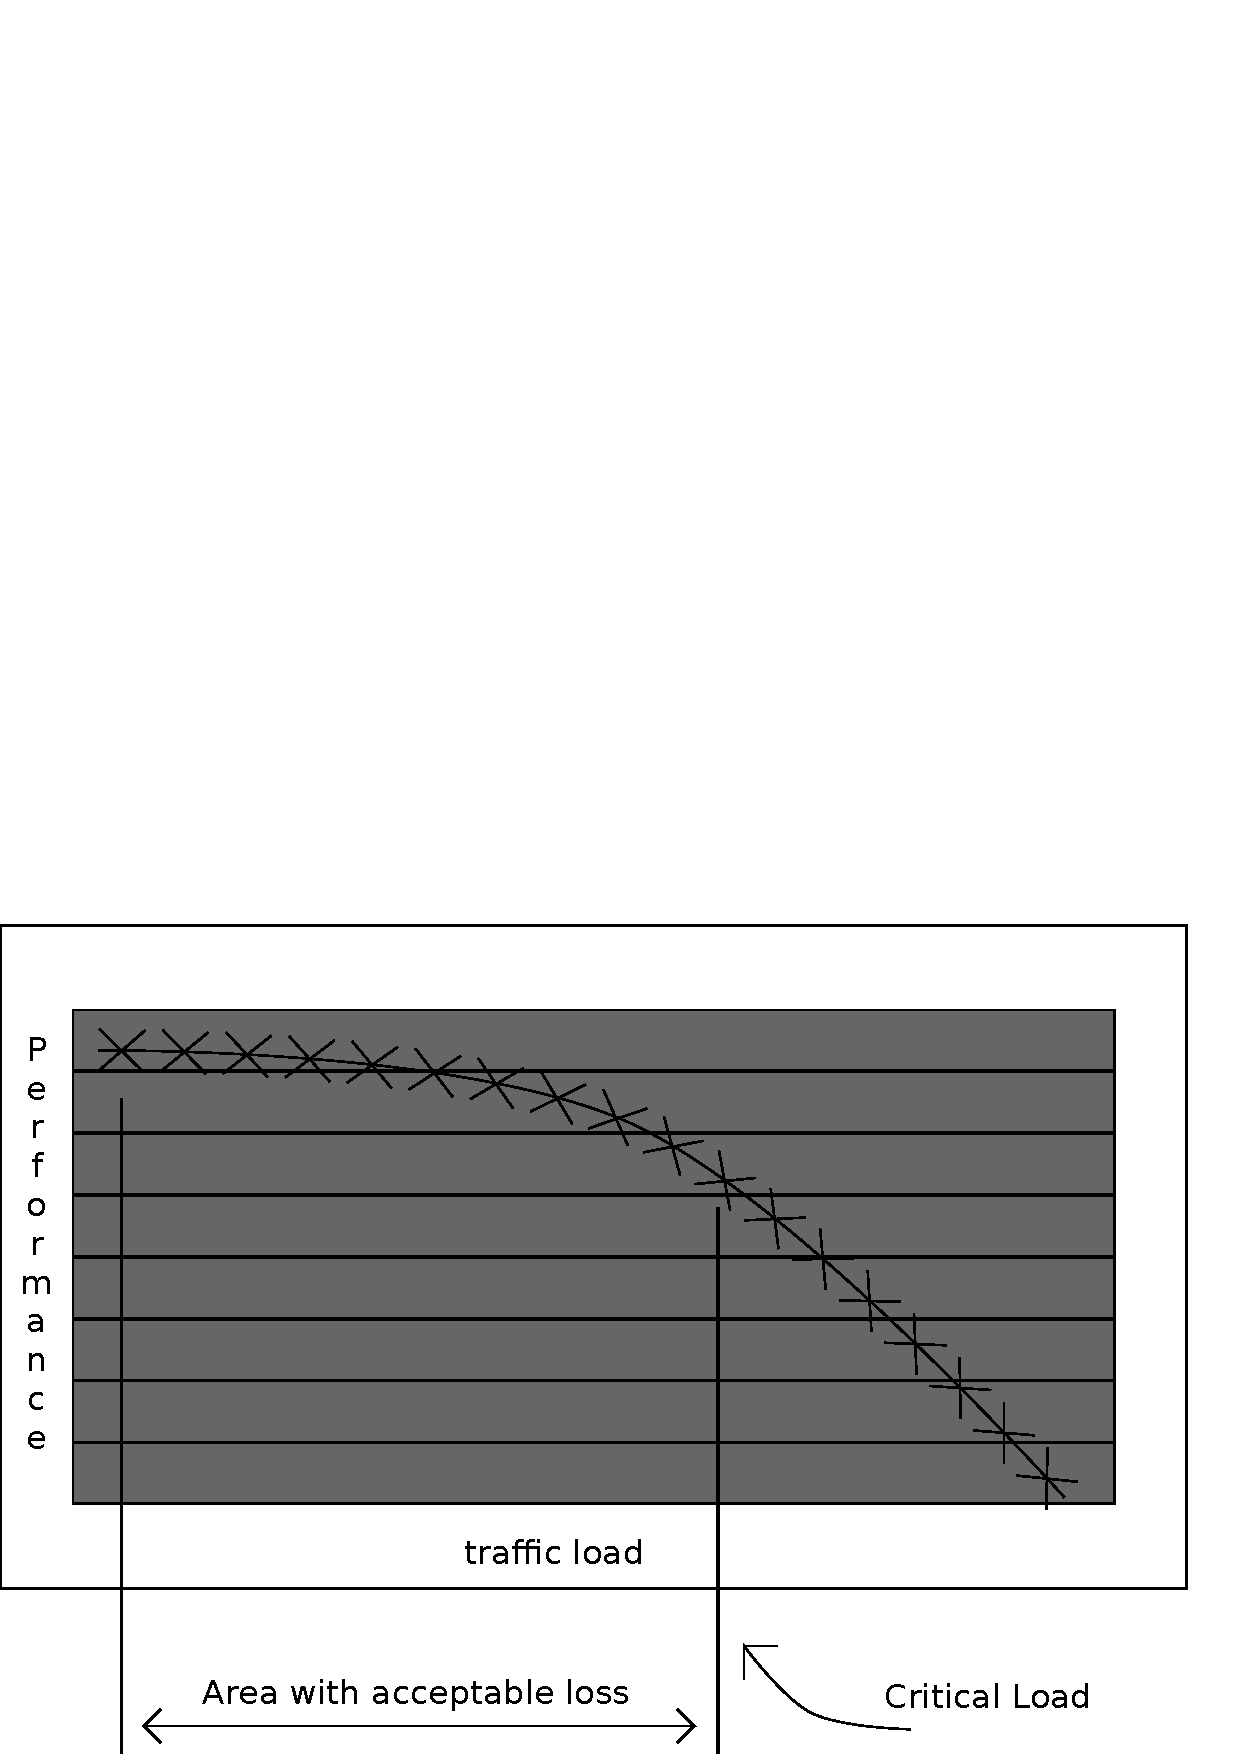
\includegraphics{goal.pdf}
      }
    \end{figure}

    Keep the load in the acceptable area as long as possible. 
  }

  \frame
  {
    \frametitle{How to?}
    \begin{figure}
      \scalebox{0.3}
      {
        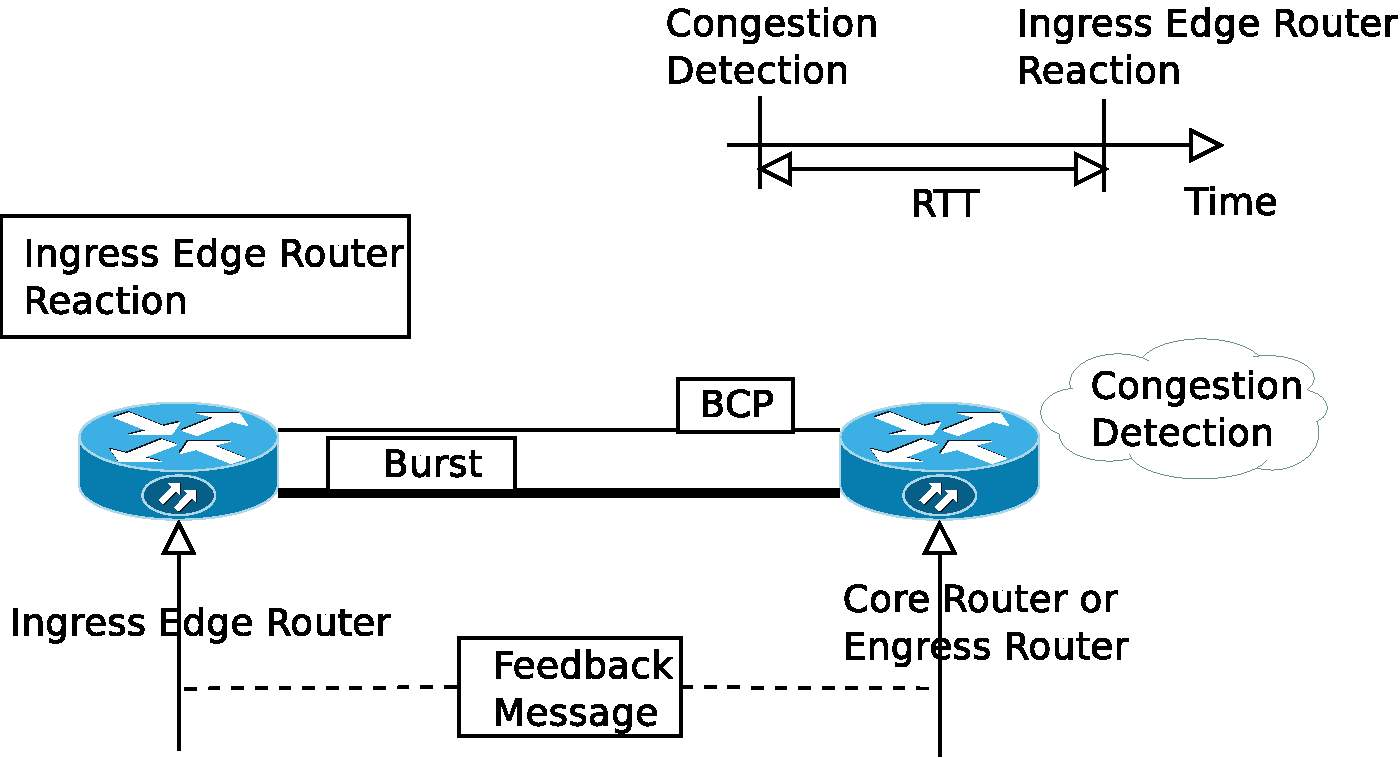
\includegraphics{how_to_congestion_control.pdf}
      }
    \end{figure}
  }

  \frame
  {
    \frametitle{How to evaluate our scheme}
    Combine simulation \& mathematical analysis: \\
    \hspace{5mm} \ding{43} Simulation Tool: \hspace{1.3mm}{\bf Opnet} \\
    \hspace{5mm} \ding{43} Analysis Method: {\bf Queuing Theory} \\

    \vspace{10mm}
    Key parameter: \\
    \hspace{5mm} \ding{43} Fairness \\
    \hspace{5mm} \ding{43} Loss Probalility \\
    \hspace{5mm} \ding{43} Retransmission times
  }

  \section{Project Plan}

  \frame
  {
    \frametitle{Project Plan}
    \begin{center}
    \begin{tabular}{|l|l|l|c|}
        \hline
        Phase & Start & Finish &Duration \\
        \hline
        Modeling & 12-Jun-2011 & 12-Jul-2011 & one month \\
        \hline
        Implemetation & 13-Jul-2011 & 20-Jul-2011 & one week \\
        \hline
        Analysis & 21-Jul-2011  & 4-Aug-2011 & two week \\
        \hline
        Report & 5-Aug-2011 & 12-Aug-2011 & one week \\
        \hline
    \end{tabular}
    \end{center}
  }
\frame{
    \frametitle{Project Plan}
    \begin{figure}
      \scalebox{0.3}
      {
          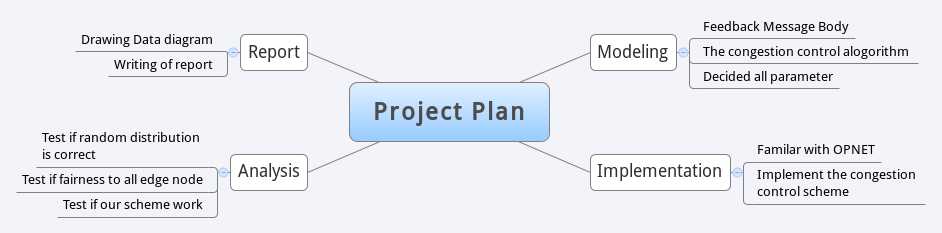
\includegraphics{project_plan.png}
      }
    \end{figure}
    }
\end{document}
